%%% PREAMBLE
\documentclass[10pt, letterpaper, twoside, openany]{book}

\usepackage{setspace}
\doublespacing

\usepackage{graphicx}
\usepackage{float}

\title{Early Detection of MCI that progresses to dementia - An Interdisciplinary Approach}
\author{
        Jomar Alcantara \\
        Department of Computer Science \\
        School of Engineering and Applied Sciences \\
        Aston University\\
        Birmingham, United Kingdom
}
\date{\today}

\begin{document}

\maketitle
\newpage
% Abstract
\section*{Abstract}
\newpage
% Acknowledgements
\section*{Acknowledgements}
Please note: An editor has not been used in the construction of this thesis.
\newpage
\tableofcontents
\newpage
\listoffigures
\listoftables

\chapter{Introduction}
\section{Introduction}
Alzheimer's Disease (AD) is a neurodegenerative disease in which, from a physiological perspective, the brain develops neurofibrillary tangles and neuritic plaques along with the deterioration and loss of cortical neurons and synapses. Whilst a definitive diagnosis of Dementia can only be produced at post-mortem, there are a number of clinical indicators from psychological perspective that can indicate dementia is present. From a clinical psychology perspective, those who have dementia demonstrate cognitive deficits such as problems with episodic and semantic memory, organizing and planning, difficulties with language, problems with executive function and visuospatial deficits \cite{McKhann2011}. In addition, these symptoms are often accompanied by emotional problems such as depression and behavioural difficulties. 
\par
AD and other forms of dementia affect a significant proportion of the geriatric population in the world today and is currently the sixth leading cause of death in the US and was named the leading killer of women in the UK. According to a recent report commissioned by the Alzheimer's Society in 2015, they estimate the prevalence of AD in the UK at approximately 815,000 people. This represents 1 in 14 of those aged 65 or over and 1 in 79 of the general population \cite{AlzheimersSociety2014}. From a financial perspective, they estimate an annual spend of £4.3 billion of which approximately £85 million is spent solely on diagnosis and that the total impact of AD (excluding the costs associated with early onset dementia) is £26.3 billion annually. Globally, this picture is a lot bleaker. Another report by Alzheimer's Disease International suggests that in 2015 there were 46 million people with a diagnosis of dementia globally and that number is expected to hit 131.5 million by 2050 \cite{Prince2015}. The report also states that the worldwide cost of AD in 2018 is estimated to be in the region of one trillon US dollars.
\par
Despite this growing problem, at present there are no drugs that improve the prognosis of those suffering with AD. All the drugs that are on the market are designed to manage symptoms. Whilst there are numerous investigational drugs in development for the treatment of AD, a larger than normal percentage (99.6\%) of these drugs fail in clinical trials (in contrast to anti-cancer drugs which have a 80\% failure rate) \cite{AlzheimersSociety2014}. Researchers have proposed that a possible reason for the lack of success is that the drugs treatments are initiated too far along in the progression of the disease and thus much of the degeneration of the brain has already taken place. It is therefore important to focus AD at it's earliest stages which some literature describes as 'Mild Cognitive Impairment (MCI) due to AD'.
\par
Current thinking suggests that the cognitive deficits associated with AD often begin before the clinical symptoms of the disease become apparent. Researchers propose that neurofibrillary tangles and other associated physiological effects of AD develop over time and alter cognitive function until a threshold is reached and clinical symptoms become more obvious \cite{Nestor2006}. The case of Iris Murdoch, who had a confirmed diagnosis of dementia, illustrates this theory well. Le et al \cite{Le2011} found, in their analysis of three writers and the novels they wrote, that Iris Murdoch's work declined subtly over time, but there was a steep drop off in the use of language in her last novel when, it is theorized, the symptoms of AD manifested themselves more significantly. If this theory holds true more generally, it should be possible to detect subtle cognitive changes in language and memory before a clinical diagnosis can be formed. One of the challenges of this approach is differentiating natural cognitive decline due to aging with decline due to a form of dementia. Albert and his team have worked to define clinical criteria which professionals can use to diagnose MCI due to AD and differentiate this from age-associated memory impairment and age-associated cognitive decline. They note that the diagnosis of MCI requires evidence of intra-individual change and optimally requires evaluation at two or more points \cite{Albert2011}.
\begin{enumerate}
	\item Concern regarding a change in cognition - A person or an informant should express concern that there is a change in cognitive ability in comparison to previous level of performance.
	\item Impairment in one or more cognitive domains - There should be evidence of lower performance in one or more cognitive domains beyond what would be expected of a person given their age and education. 
	\item Preservation of independence in functional - Whilst persons with MCI are expected to be able to maintain independence, it is common to experience mild problems in complex functional tasks which they may have been able to perform previously. This might mean that they take more time or be less efficient at completing these tasks, or it may be that may make more mistakes.
	\item Not demented - The deterioration should be mild to the point that there is no significant loss of functioning in social or occupational contexts.
\end{enumerate}
In addition to meeting the above criteria, a clinician must rule out other conditions or factors that could account for the decline in cognition with the goal to increase the likelihood that the underlying cause of this decline is dementia. 
\par 
Many researchers have studied the early detection of MCI. These studies usually follow two main approaches. The analysis of biomarkers and the examination of patients who have demonstrated decreasing cognitive abilities. The first approach yields reliable results in the detection of AD in its moderate and advanced states but does not perform well during the early stages of the disease. The second approach has gained more attention in recent years, due to the fact that in clinical practice it has shown promise in the early detection of AD. In addition, the analysis of the decline of cognitive abilities is comparatively inexpensive and less invasive that the first approach which commonly requires the collection of a sample of cerebro-spinal fluid which is painful for the patient involved. 
\par
One of the most common ways in which clinicians traditionally make an early diagnosis of dementia is through the use of the Mini Mental State Examination (MMSE) \cite{Folstein1975}. The MMSE is a brief questionnaire consisting of eleven questions which tests cognitive aspects of mental function and requires only 5-10 minutes to administer \cite{Folstein1975}. The MMSE is chosen due to it's effectiveness at assessing a person's cognitive mental state at a specific point in time, as well as being as sensitive to changes as a more detailed and complex assessment such as the Wechler Adult Intelligence Scale \cite{Folstein1975}. Whilst the MMSE is useful as a brief screening tool it has it's limitations. The MMSE was not specifically created to screen for dementias and therefore does not interrogate key aspects of cognitive impairment known to be affected in dementia. It also has limited value in assessing under-educated subjects and a meta-analysis on the effectiveness of the MMSE as a diagnostic tool for dementia showed that it's accuracy was low (sensitivity between 78.4\% and 85.1\% and specificity between 81.3\% and 87.8\%). As the MMSE has been shown to have low accuracy specifically in the diagnosis of dementia, it becomes necessary for professionals to employ the use of other tools or measures such as the Free Cued Selective Reminding Test (FCSRT) \cite{Grober2010} or the Montreal Cognitive Assessment (MoCA) \cite{Davis2015}. 
\par 
These tests have the benefits of being much more accurate at diagnosing cognitive impairment and discriminating between dementia and other types of cognitive impairment at the cost time and training of psychological professionals such as clinical psychologists in administering these tests. However, the utility of diagnosing dementia at the point where clinical intervention is warranted is limited because at this stage both psychological and pharmacological interventions have been shown to not be effective \cite{Prince2015}. In order to further our understanding of the progression of dementia it is important to detect the signs of dementia before they are clinically apparent. 
\par
The two main ways in which diagnosis is performed is through assessment of memory and language. Tests of memory are classically among the most accurate ways of diagnosing dementia, however these tests suffer from the same reliance on clinicians to administer these tests in a clinical setting. Language however is a lot easier to collect and can be done in more naturalistic settings. As with memory, these tests can be done over time and would be able to chart a patients language degeneration over time. Given that language is less intrusive to test and requires a lot of the cognitive processes that may be impacted by AD, a lot of research has focused on measure decline in the use of language in those with AD. There are a number of difficulties to watch out for with this approach. There are a wide number of factors that are involved in language degeneration in the elderly, and consequently there will be an expected amount of variability between subjects. The administration of such tests may induce nervousness and discomfort which may impact performance, and also repeatedly administering the same language tests for differences over time may be confounded by improved performance at tasks via practice effects. However, there is enough promise in this approach such that it could help further our understanding of the disease, it's progression and the parts of the brain affected in the early stages.
\par
According to the DSM 5 \cite{AmericanPsychiatricAssociation2013}, those with mild dementia suffer from noticeable word finding difficulty. They may substitute general terms for more specific terms and may avoid the use of specific names of acquaintances. There may be grammatical errors involving subtle omission or incorrect use of articles, prepositions, auxiliary verbs, etc. Those who have progressed from Mild to Major depression also have difficulties with expressive or receptive language. They will often use general-use phrases such as "that thing" and "you know what I mean" and prefers general pronouns rather than names. With severe impairment, sufferers may not even recall names of closer friends and family. Idiosyncratic word usage, grammatical errors, and spontaneity of output and economy of utterances occur. Echolalia (meaningless repetition of another person's spoken words) and automatic speech typically precede mutism. With the wide range of deficits someone with AD can suffer, it makes sense to try to categorise these deficits in some way.
\par
One of the most famous pieces of research on the topic of language decline in dementia was by Berisha and Liss who examined speeches and public interviews of former US president Ronald Reagan \cite{Berisha2015}. They found that Reagan's speeches towards the end of his presidency suffered from difficulties in word-finding, inappropriate phrases and uncorrected sentences which are hallmarks of language deterioration associated with Alzheimer's Disease. It turned out later to be the case that he had Alzheimer's Disease. Another classical study by Snowdon et al looked at whether linguistic ability in early life was associated with cognitive function and AD in later life \cite{Snowdon1996} . They found that idea density (defined as the number of expressed propositions divided by the number of words) was a key predictor in predicting whether nuns would go on to develop AD in later life. They found that those who would go on to develop AD all had low idea density in early life and they found no AD present in those with high idea density in early life. As we can see, just with these two pieces of research the range of language deficits in those who suffer with AD are extremely variable and can differ from patient to patient as the disease progresses. The consensus among researchers that this language degeneration is typically accelerated by the presence of dementia \cite{Berisha2015} and that a potential indicator of dementia is the rate of change in which the decline occurs relative to a fixed point in time rather than a comparison across a cohort of individuals. 
\par
Emery \cite{Emery2000} completed a literature review looking at all the potential language deficits that could exist in those with AD and / or MCI. She divided these deficits into four levels of language: Phonology, Morphology, Syntax and Semantics. She proposed that language and the processes involved in language are hierarchical in nature and that language moves from simple units of construction (Phonology and Morphology), and build layers of complexity and sophistication (Syntax and Semantics). She found that people with AD generally had intact Phonology and Morphology but more impaired Syntax and Semantics. She asserted that the language forms we learn last are the first to deteriorate as we generally learn language in small simple units initially and build syntax and complexity as we are more comfortable with language. However it is important to note that different variants of dementia show different deficits in terms of language productions. Regardless, dividing language in this way is useful as it allows us to detect deteriorations in different parts of language usage and therefore may provide a way of discriminating between different forms of dementia. 
\par
It is clear from both the clinical diagnostic criteria and supporting research that language is impacted in those with AD. However, whilst there is a move towards research aimed at looking more specifically at MCI we currently lack the measures that are sensitive enough to detect MCI. Given that we know language is affected before a clinical diagnosis of dementia is usually made \cite{Berisha2015, Snowdon1996, Le2011}, it makes sense to explore whether language on it's own can provide markers that may indicate a cognitive impairment that could progress to dementia. The field of machine learning and natural language processing has been suggested as a way to improve the accuracy and lessen the human cost of this research as well as provide new insights into the difficulties that AD suffer in terms of language decline \cite{Boschi2017}.
\par 
In 2009, the UK's Department of Health designed it's National Dementia strategy and as part of this made early diagnosis and support one of it's key priorities \cite{England2009}. A lot of work has gone into trying to find ways of improving the early diagnosis of Alzheimer's Disease (AD) and Mild Cognitive Impairment (MCI) with research focused on two areas - identifying biological markers and analyzing the cognitive decline of those who are suspected to have the disease \cite{Taler2008}. As described above, the numbers of those suffering from AD and MCI are going to increase as the population ages \cite{Prince2015} and thus it is important that we utilize technology wherever possible to aid clinicians in the detection of MCI and AD. At the present time diagnostic assessment is typically conducted at memory clinics by trained clinicians \cite{Boschi2017} and whilst it is not possible to provide a definitive diagnosis until after death. 

I theorize that we may be able to enable an earlier diagnosis of those with MCI and AD using samples of spontaneous speech, natural language processing (NLP) and machine learning (ML).
\par
There is a large body of research that looks at the decline in language in those with MCI and AD \cite{Taler2008, Boschi2017}. However there is conflicting evidence in these studies about which declining language factors are associated of MCI and AD \cite{Taler2008, Boschi2017}. Research therefore should look at these features in more detail and a clarification of this currently disorganised picture should go some way to helping researchers further understand the disease and it's progression. Another area of focus for research of this nature is the process of collecting appropriate language samples. Whilst collecting samples of language is comparatively unintrusive, researchers recognise that these samples require a rich sample of language that potentially cannot be generated by tasks such as the picture description task. Therefore, it would be useful to explore whether spontaneous discourse such a semi-structured interview, has the ability to put pressure on both the cognitive and linguistic systems in the same way as traditional cognitive tests such that it might be able to distinguish between healthy controls, those with MCI and those with AD. There is some evidence to support this. Berisha et al \cite{Berisha2015}, has shown through a longitudinal language analysis of spontaneous speech that there are marked differences in this process between those who would go on to have a diagnosis of AD and a healthy control. 
\par
The potential impact of this research in this area is immense. Research has shown that early diagnosis of people with AD or MCI improves sufferers quality of life and can, in some cases, slow the progress of the disease. Early diagnosis can increase the number of research opportunities for understanding the early stages of dementia and how the disease progresses so that more research can be conducted which may, in the future, lead to new treatments and other interventions.
\par
In chapter 2 Background and Related Work
\par 
In chapter 3 Systematic Review of NLP and Machine Learning Research
\par 
In chapter 4 Delphi Methodology and developing consensus on how best to collect language samples using technology
\par 
In chapter 5 Development of a pipeline that processes language data accurately
\par 
In chapter 6 Analysis of DementiaBank dataset
\par
In chapter 7 Pilot study of the methodology developed
\par 
Finally, in chapter 8. I discuss conduct a general discussion of the results of my research. I also think about the strengths and weaknesses of my work and suggest ways in which the research have been improved. Lastly, I look at a number of areas for future work which can build on this research.


\chapter{Background and Related Work}
\section{Introduction}
Here is the text of your introduction.

\begin{equation}
    \label{simple_equation}
    \alpha = \sqrt{ \beta }
\end{equation}

\subsection{Subsection Heading Here}
Write your subsection text here.


\section{Conclusion}
Write your conclusion here.



\chapter{Systematic Review of NLP and Machine Learning Research}
\section{Introduction}
Here is the text of your introduction.

\begin{equation}
    \label{simple_equation}
    \alpha = \sqrt{ \beta }
\end{equation}

\subsection{Subsection Heading Here}
Write your subsection text here.


\section{Conclusion}
Write your conclusion here.


\chapter{Delphi Methodology and developing consensus on how best to collect language samples using technology}
\section{Introduction}
Here is the text of your introduction.

\begin{equation}
    \label{simple_equation}
    \alpha = \sqrt{ \beta }
\end{equation}

\subsection{Subsection Heading Here}
Write your subsection text here.


\section{Conclusion}
Write your conclusion here.


\chapter{Development of a pipeline that processes language data accurately}
\section{Background}
There has been a significant research in the area of language deterioration as a means of detecting Alzheimer's Disease. This usually takes the form analysis of speech recorded as part of a cognitive assessment such as the Picture Description Task \cite{Orimaye2014,Fraser2015}. Given that language samples are relatively easy to collect, research has moved towards analysis of spontaneous speech. An good example of this type of research is the study conducted by Berisha and Liss which looked at the differences in language use between two US presidents, Ronald Reagan (who would go on to receive a diagnosis of Dementia) and George H.W. Bush who acted as a matched control based on Age \cite{Berisha2015}. They found several differences in language use which they felt acted as indicators of Reagan's difficulties with language due to dementia. These significant differences were in the number of unique words used per speech, the use of non-specific nouns and fillers and low-imageability verbs \cite{Berisha2015}. 
\par   
This study replicates work done by Berisha and Liss and extends this by adding Donald Trump as an alternative, more appropriate comparison to Ronald Reagan as he is much closer in age than George H.W. Bush. This experiment will look at the features originally identified by Berisha and Liss, as well as any others that have potential as discussed in the literature review above. 
\section{Methods}
I took 46 transcripts of Ronald Reagan’s (RR) press conferences from 1981 to 1988 and compared them with 134 press conferences by George H. W. Bush (GHWB) and 29 press conferences conducted by Donald J. Trump (DJT).  I analyzed transcripts for lexical features shown to change longitudinally with dementia  (for a comprehensive review of these, see the literature review above). For this collection of documents, I generated a number of features which looked at a number of different aspects of each document. These features encompassed, word level, sentence level and document level features and included a number of features contained in the study by Berisha and Liss with the aim of replicating and extending on their findings. These findings were. number of unique words, non-specific nouns and fillers and low imageability (LI) verbs. Imageability is characterized, according to Berisha and Liss, as the ease with which a term gives rise to a sensory .mental image. I compared the trends described in the transcripts of RR and GHWB, but also included DJT. Berisha and Liss originally made the comparison as it GHWB (GHWB - age at the start of presidency - 64 years, 222 days) was the closest match to RR in terms of age (RR  - age at the start of presidency, 69 yeaars and 349 days). However, with the inauguration of Trump, he now is the closest comparible president in terms of age (DJT - age at the start of presidency - 70 years, 220 days). It would be interesting to look at a comparison of RR and DJT to see whether the comparisons made by Berisha and Liss hold true with this more appropriate match (in terms of age). DJT as with GHWB has no known diagnosis of AD. I used the press conference transcripts in the American Presidency Project (APP) archive as a data source for this project. The APP is a comprehensive and organized searchable database of presidential documents, including transcripts of speeches, transcripts of news conferences, and other public documents.
\subsection{Pre-processing}
To generate the files necessary for analysis, I downloaded each transcript and performed the following changes. I omitted the prepared statement by the president and any speech by other individuals. I started each transcript at the beginning of the first answer to a question. I filtered any annotations that were added to the transcript, including any references or clarifications, and any laughter. It's worth noting that there appears to be a difference in how 'hesitations' were marked down between each president, for RR hesitations were marked by a single hyphen whereas for GHWB hesitations are marked by a double hyphen. In order to maintain consistency when parsing through the documents, I have changed both types of hesitation to be marked by a single hyphen. I also omitted one word sentences as this data would, from a theoretical perspective, not be relevant for language analysis. I did not control for the length of the document, but generated features which would normalise by the length of the document. I therefore was able to include all press conferences by both Ronald Reagan and George H.W. Bush where there was a question and answer session conducted at least in part by the sitting president (2 press conferences of GHWB were ommited due to a lack of a question and answer session).
\subsection{Feature Selection}
We calculated the following features for each transcript in turn using the NLTK (see section 2 for a description) \cite{Bird2009} and Python. 
\par 
\subsubsection{Measures of lexical variation}
We constructed two features of lexical variation. Firstly we looked at the number of unique words. To do this we were able to split each transcript into individual words and changed them to lowercase using NLTK and were then count the number of unique words that appeared in each transcript. We also used the TTR formula (see section 2 for a description) for a feature that measures lexical diversity independent of sample size \cite{Richards1987}. 
\subsubsection{Fillers, Non-Specific Nouns and LI Verbs}
For these features, we counted the number of occurrences for different categories (see table for list of categories tracked and the words counted). The features were used by Berisha and Liss in their research \cite{Berisha2015} and were taken from work done by Bird et al \cite{Bird2000}. 

\begin{table}[H]
	\begin{center}
	\begin{tabular}{ | p{3cm} | p{6cm} |}
		\hline
		Category & Words \\ \hline
		Fillers & \textit{"well", "so", "basically", "actually", "literally", "um", "ah"} \\ \hline
		Non Specific Nouns & \textit{"something", "anything", "thing", "everything"} \\ \hline
		LI Verbs & \textit{"be", "come", "do", "get", "give", go", "know", "look", "make", "see", "tell", "think", "want"} \\ \hline

	\end{tabular}
	\caption{\label{tab:table-name}Categories and Words Counted}
	\end{center} 
\end{table}

\subsubsection{Usage of parts of speech}
This section involves using a Part of Speech tagger (PoS) which analyses a sentence and assigns a 'tag' to each word based on the function the word has in a sentence. At a basic level this can be divided into the eight defined parts of speech: 'nouns', 'pronouns', verbs', 'adjectives', 'adverbs', 'conjunctions', 'prepositions' and 'interjections' but can be further subcategorised. We used the PoS tagger built into NLTK to tag each transcript in turn and used these the counts from each of these eight categories in our analysis. In addition to frequency counts we also normalised these features by dividing the frequency count by the number of words in the document to take into account transcript length.

\section{Results}
One of the most important thing to note is the wide variety of samples between the three presidents and also the varying timescales. RR participated in 46 press conferences over eight years (an average of 5.75 a year) which is the fewest number of press conferences given by an American president during their term of office. GHWB participated in 136 press conferences over four years (an average of  34 a year) and DJT participated in 29 press conferences to date (an average of 19.3 per year). Equally, there are variances in the average number of words. RR produced an average of 3424 words per conference compared to 2608 by GHWB (unpaired t = 4.434, p\textless 0.001) and DJT at 1849 words (unpaired t = 6.524, p\textless 0.001).
\begin{table}[H]
	\begin{center}
	\begin{tabular}{ | p{3cm} | p{1.5cm} | p{1.5cm} | p{1.5cm} |}
		\hline
		& RR & GHWB & DJT \\ \hline
		Total Words & 3423.91 (416.42) & 2607.72 (1210.38) & 1848.65 (1549.38) \\ \hline
		Unique Words & 894.13 (85.15) & 667.76 (218.67) & 481.82 (221.29) \\ \hline
		Non Specific Nouns & 12.72 (4.63) & 6.78 (4.32) & 7.41 (8.75) \\ \hline
		LI Verbs & 124.22 (17.89)& 103.45 (51.87) & 84.48 (75.78) \\ \hline
	\end{tabular}
	\caption{\label{tab:table-name}Means and Standard Deviations of important features}
	\end{center} 
\end{table}

In terms of unique words, we found that RR used significantly more unique words, non-specific nouns and low imageability verbs than GHWB and DJT (see Table 3.3). Some of these differences are due to the length of the sample, particularly in the case of DJT where his average sample is almost half the sample of RR. It could also be said that this could be down to differences in linguistic abilities or speaking style \cite{Berisha2015, Le2011}. However, we can certainly see that as controls GWHB and DJT are comparative in relation to non-specific nouns and LI verbs. 

\begin{table}[H]
	\begin{center}
	\begin{tabular}{ | p{3cm} | p{1.5cm} | p{1.5cm} | p{1.5cm} |}
		\hline
		& RR v GHWB & RR v DJT & GHWB v DJT \\ \hline
		Total Words & \textbf{4.434***} & \textbf{6.524***} & \textbf{2.899**} \\ \hline
		Unique Words & \textbf{6.832***} & \textbf{11.403***} & \textbf{4.137***} \\ \hline
		Non Specific Nouns & \textbf{7.877***} & \textbf{3.426**} & -0.574 \\ \hline
		LI Verbs & \textbf{2.656**} & \textbf{3.420***} & 1.628 \\ \hline
		\multicolumn{4}{@{}p{1.5in}}{\footnotesize * denotes p\textless 0.05} \\
		\multicolumn{4}{@{}p{1.5in}}{\footnotesize ** denotes p\textless 0.01} \\
		\multicolumn{4}{@{}p{1.5in}}{\footnotesize *** denotes p\textless 0.001} \\
	\end{tabular}
	\caption{\label{tab:table-name}RR T-tests vs GWB and DJT}
	\end{center} 
\end{table}

We then looked at the data from a longitudinal perspective as we are interested seeing whether we can track various language variables and their progress over time. We ran a number of Pearsons correlations with transcript index number as a time reference and the dependant variables (Table 3.4).  For our controls, we found them to be stable for the most part with the main highlights being a decrease in Adverb usage for DJT (R=-0.36, p=0.049) and a steady but not severe decline in a number of variables for GWHB, namely total word count, unique words, low imageability words and verb usage.
\par 
For RR, his decline is more marked and more widespread through his language use. We noticed an significant increase in adverb (R=0.41, p=0.004) and pronoun usage (R=0.65, p\textless0.001), as well as a slight usage increase in Non-specific nouns(R=0.30, p=0.03). There was a highly significant decrease in number of unique words (R=-0.56, p\textless0.001) and noun usage (R=-0.70, p\textless0.001). Also very significant decrease in adjective usage (R=-0.40, p=0.005) and a significant decrease in total word count (R=-0.31, p=0.03). 

\begin{table}[H]
	\begin{center}
	\begin{tabular}{ | l | p{1.5cm} | p{1.5cm} | p{1.5cm} |}
		\hline
		& RR & GHWB & DJT \\ \hline
		Word Count & \textbf{-0.31*} & \textbf{-0.21*} & 0.08 \\ \hline 
		Unique Words & \textbf{-0.56***} & \textbf{-0.25**} & 0.16 \\ \hline
		Non Specific Nouns & \textbf{0.30*} & -0.08 & -0.03 \\ \hline
		LI Verbs & -0.19 & \textbf{-0.20**} & 0.02 \\ \hline
		Nouns Normalised & \textbf{-0.70***} & -0.03 & 0.14 \\ \hline
		Verbs Normalised & \textbf{0.36**} & \textbf{0.24***} & -0.03 \\ \hline
		Adjectives Normalised & \textbf{-0.40**} & 0.08 & -0.34 \\ \hline
		Adverbs Normalised & \textbf{0.41***} & 0.02 & \textbf{-0.36*} \\ \hline
		Pronouns Normalised & \textbf{0.65***} & 0.13 & 0.07 \\ \hline
		\multicolumn{4}{@{}p{1.5in}}{\footnotesize * denotes p\textless 0.05} \\
    	\multicolumn{4}{@{}p{1.5in}}{\footnotesize ** denotes p\textless 0.01} \\
    	\multicolumn{4}{@{}p{1.5in}}{\footnotesize *** denotes p\textless 0.001} \\
	\end{tabular}
	\caption{\label{tab:table-name}Pearson Correlations for Features}
	\end{center} 
\end{table}

\section{Discussion}
President Reagan received his diagnosis of AD in August 1994 but using transcripts of speeches he made in his two terms as President (January 1981 - January 1989) we have be able to identify certain changes in his use of language that we might ascribe to the onset of MCI and early AD. Despite differences in our methodology, our research supports the findings of Berisha and Liss in that we both find a significant decrease in unique words over time and an increase in non-specifc noun usage. Compared to our controls (GWHB andDJT), we find some slight trends with GWHB but no such trends with DJT in his speech albeit his samples of speech span a shorter amount of time.
\begin{figure}[H]
	\centering
	\begin{minipage}[b]{0.4\textwidth}
		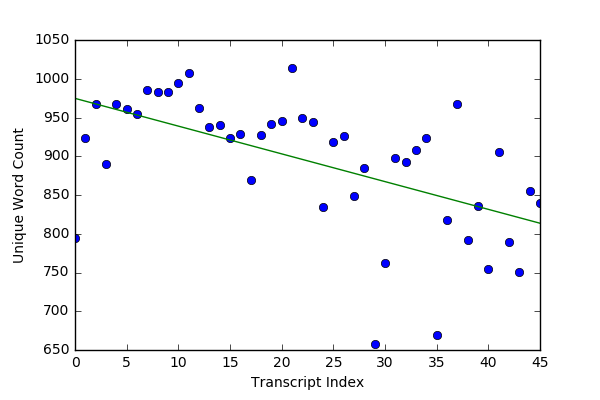
\includegraphics[width=190px, height=140px]{images/RRUniqueWords.png}
		\caption{Ronald Reagan - Unique Words over time}
	\end{minipage}
	\hfill
	\begin{minipage}[b]{0.4\textwidth}
		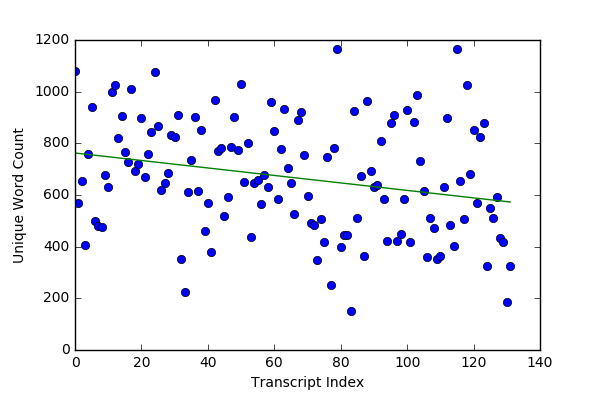
\includegraphics[width=190px, height=140px]{images/GWHBUniqueWords.png}
		\caption{George H.W. Bush - Unique Words over time}
	\end{minipage}
\end{figure}

\begin{figure}[H]
	\centering
	\begin{minipage}[b]{0.4\textwidth}
		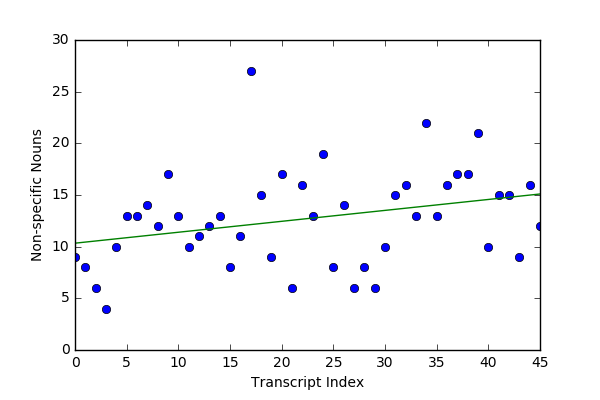
\includegraphics[width=190px, height=140px]{images/RRNSNouns.png}
		\caption{Ronald Reagan - Non-specifc Nouns over time}
	\end{minipage}
	\hfill
	\begin{minipage}[b]{0.4\textwidth}
		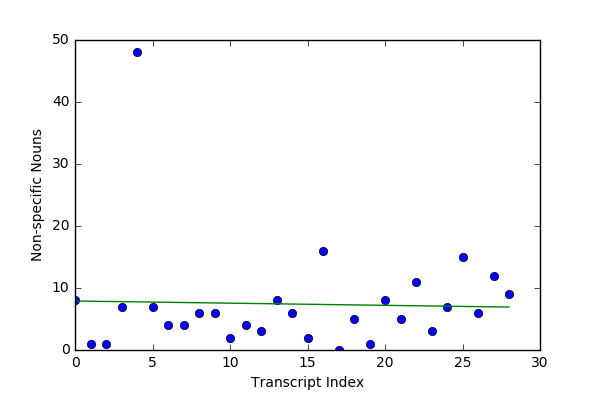
\includegraphics[width=190px, height=140px]{images/DJTNSNouns.png}
		\caption{Donald J. Trump - Non-specific Nouns over time}
	\end{minipage}
\end{figure}

A criticism of Berisha and Liss's work is the problems they had with normalising the transcripts in terms of length. This was also a problem in the work of Garrard et al \cite{Garrard2005, Le2011}. Whilst it is important to control for outliers, there are other ways in which we can control for length of sample.  
\par 
Interestingly, when we normalised the various types of words used by the presidents we found some interesting patterns that further differentiated RR from the controls. Whilst Non-specific nouns increased over time, we found that noun usage in general significantly decreased and pronouns increased similarly significantly. The increase in pronoun for those with early AD has been identified in literature, although there are only a few studies that explore this \cite{Almor1999, Wendelstein2015}. Wendlestein et al propose that the increased used of pronouns is an expression of an impaired ability to adapt language to the listener's needs \cite{Wendelstein2015}. Almor et al attributed this reliance on pronouns due to a impaired working memory \cite{Almor1999}.
\par 
The decrease in overall noun usage has also been identified as a feature. Jarrold et al found that AD patients would use more pronouns, verbs and fewer nouns than controls \cite{Jarrold2014}. Wendlestein in their investigations into noun usage found that decreased later on in AD progression and was unaffected in the pre-clinical stages of AD \cite{Wendelstein2014}. Our results are supported by existing literature and this potentially means that language analysis in the way we have structured it may have diagnostic or prognostic properties.

\begin{figure}[H]
	\centering
	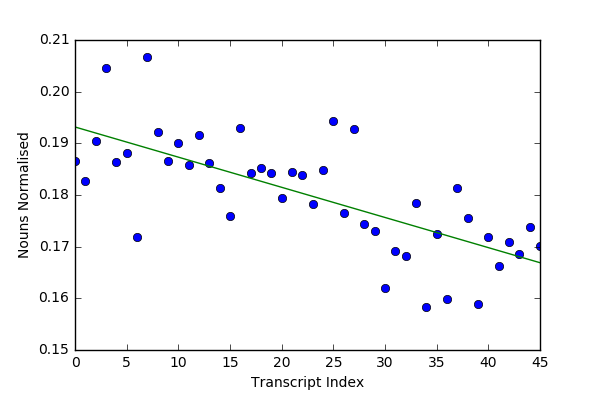
\includegraphics[width=240px, height=150px]{images/RRNounsNormalised.png}
	\caption{Ronald Reagan - Nouns Normalised over time}
\end{figure}

\begin{figure}[H]
	\centering
	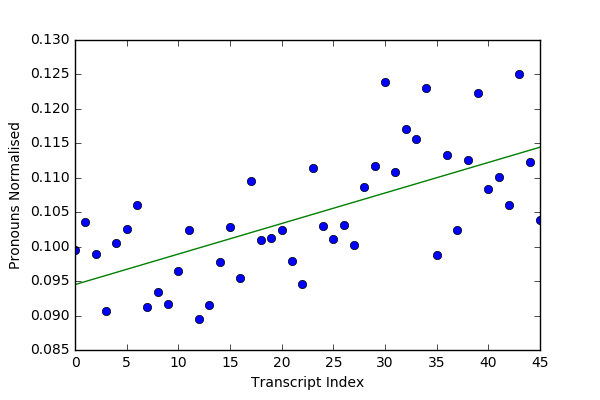
\includegraphics[width=240px, height=150px]{images/RRPronouns.png}
	\caption{Ronald Reagan - Pronouns Normalised over time}
\end{figure}
 
There are limitations of this research. Whilst in terms of age, DJT is certainly more suitable as a control to match with RR, in some ways they held very different styles of press conferences in that RR preferred to do solo press conferences and DJT has shown a preference for doing joint press conferences which have an impact on the amount of language produced. This artifact of the data is in itself notable as it illustrates the problems we may have with smaller amounts of speech. Also, the problem of finding an appropriate control is a common one in this domain. Given that those with MCI and early dementia have such variable presentations, it might prove of limited value in matched pairs design. 
\par 
With further work, it is not feasible to the vast array of samples over a timeframe, as we have had with the president corpus and so it would be worth exploring how the quality of these predictions might lessen when faced with considerably fewer samples and over a smaller time period. It would also be worth extending this research further to encompass more of the linguistic features Fraser used in her work \cite{Fraser2015} to see if there are any further insights to be gained. In addition, this replication and extension has demonstrated the potential utility of using longitudinal data as a means of comparing language use of a person at two or more time periods and using this information as a diagnostic aid for MCI and therefore more work would be helpful from a longitudinal perspective to see if this approach may be valid in moving towards a solution for this particular problem. 
\par 
The results of this work show that we can track a person's use of language through time in a number of ways, and it is possible for an individual to be his or her own control. This is important as it means the heterogenous nature of the MCI population does not impact results as much as if we were comparing those with MCI to controls. Equally, it would be helpful to have controls to ascertain what would be usual to expect in the decline of language in a healthy older adult. 


\chapter{Analysis of DementiaBank dataset}
\section{Introduction}
Here is the text of your introduction.

\begin{equation}
    \label{simple_equation}
    \alpha = \sqrt{ \beta }
\end{equation}

\subsection{Subsection Heading Here}
Write your subsection text here.


\section{Conclusion}
Write your conclusion here.


\chapter{Pilot study of the methodology developed}
\section{Introduction}
Here is the text of your introduction.

\begin{equation}
    \label{simple_equation}
    \alpha = \sqrt{ \beta }
\end{equation}

\subsection{Subsection Heading Here}
Write your subsection text here.


\section{Conclusion}
Write your conclusion here.


\chapter{General Discussion, Conclusions and Future Work}
\section{Introduction}
Here is the text of your introduction.

\begin{equation}
    \label{simple_equation}
    \alpha = \sqrt{ \beta }
\end{equation}

\subsection{Subsection Heading Here}
Write your subsection text here.


\section{Conclusion}
Write your conclusion here.


\bibliographystyle{unsrt}
\bibliography{main.bib}

\end{document}